
% \listoftodos
% \todototoc

\section{Introduction}


% \todo{poderia trocar esses surveys por mais novos ou menos preditivos e mais acertvivos}

% A survey released by Gartner estimated about 20 billion devices connected to the
% Internet by 2020, many of them through the IoT \cite{gartner_forecast_2017}.
% More recently, Statista predicted that the total number of such devices will
% reach 38 billion by 2025, and 50 billion by 2030 \cite{statista-iot}.
The Internet of Things (\iot) brings together a wide variety of devices,
including mobile, wearable, consumer electronics, automotive, and sensors of
various types.
% 
Such devices can either be accessed by users through the Internet or connect
to other devices, servers, and applications
with little human intervention or supervision
\cite{Tahsien2020,abane2019,haddadpajouh2019survey,Shanbhag2015}.
% 
Security and privacy is a major concern in the \iot, specially regarding
% devices like smart home assistants and wearable
devices having access to user personal data like
location, health, and many other sensitive data \cite{sengupta2020comprehensive}.
% 
Furthermore, if compromised such devices can also be used to attack other
devices and systems, steal information, cause immediate physical damage or
perform various other malicious acts \cite{Kolias2017mirai}.
% 
As an additional concerns, \iot devices likely have long lifespan, less frequent
software patches, growing diversity of technologies combined with lack of
control over the software and hardware of such devices by the host organization
(where the device is deployed) considerably increases the attack surface.

% A study reveals that nearly $20\%$ of organizations have experienced at least one
% IoT-based attack in the last three years.
% The study shows that most organizations have no control over the origin and
% nature of software and hardware used by the connected devices.
% To protect against these threats, the IoT industry's spending on security is
% estimated to be around USD $\$\,3.1$ billion in 2021 \cite{gartner_it_glossary_2018}, 
% which includes the development of tools
% and services to improve asset discovery and management, software security
% evaluation, hardware % testing 
% and penetration testing.

% i.e. 'id est', which means "that is."
% e.g. 'exempli gratia', which means "for example."
% {\color{red} muito próximo de \cite{Cassales2019a}}
Because most \iot devices have limited resources (i.e., battery, processing,
memory, and bandwidth), configurable and expensive algorithm-based
security techniques may not fit \cite{Zhou2017}.
Machine Learning (ML) techniques have been studied for years to detect attacks
from known patterns or to discover new attacks at an early stage
\cite{buczak2016survey,mitchell2014survey}.
A recent survey \cite{Tahsien2020} shows that ML based methods are a
promising alternative which can provide potential security tools for the \iot
network making them more reliable and accessible than before.

Despite the promising use of ML to secure \iot systems, studies in the
literature \cite{buczak2016survey,mitchell2014survey,Tahsien2020} are limited to
traditional ML methods that use static models of traffic behavior.
% With traditional ML methods, the data set is static and can be traversed
% repeatedly, and the detection of new attack patterns requires a new cycle of
% training, testing, and dissemination of new models.
Most existing ML solutions for network-based intrusion detection cannot maintain
their reliability over time when facing evolving attacks \cite{Viegas2019}.
Unlike traditional methods, stream mining algorithms can be applied to intrusion
detection with several advantages, such as:
\begin{enumerate*}[label=(\emph{\roman*})]
    \item processing traffic data with a single read;
    \item working with limited memory (allowing the implementation in small
    devices commonly employed in edge services);
    \item producing real-time response; and
    \item detecting novelty and changes in concepts already learned.
\end{enumerate*}

% Nao tinha mencionado quais previous works...
% {\color{red} %This paper elaborates on the previous work in the following aspects.

{\color{red} Adicionar referencias e relacionados. Argumentar que além de \nids,
\nd para \iot tem outras aplicações}

Given the recent use of Data Stream Novelty Detection (\nd) in network data
streams, this paper shows the effects of adapting these mechanisms to edge
services for use in \iot environments.
Our proposal, \mfog, instantiated and experimentally validated the \arch
architecture \cite{Cassales2019a} employed the \nd algorithm \minas
\cite{Faria2013Minas,Faria2015minas} (as it was already tested in a similar \iot
scenario) on a distributed system composed of small devices with limited
resources on the edge of the network.
% Our implementation can be fully executed on the edge, thus avoiding any dependency
% and high latency of cloud resources.
% We proposed and implemented dMINAS, a distributed extension
% of MINAS \cite{Faria2016minas} (a novelty detection for data streams).
We evaluated through experimental methodology, how the distribution of
% the chosen novelty detection algorithm
\minas
affects the capability to detect changes (novelty) in
traffic patterns, and the impact on the computational efficiency.
Finally, some distribution strategies and policies for the data stream
novelty detection system are discussed.
% }

\begin{figure}
    \centering
    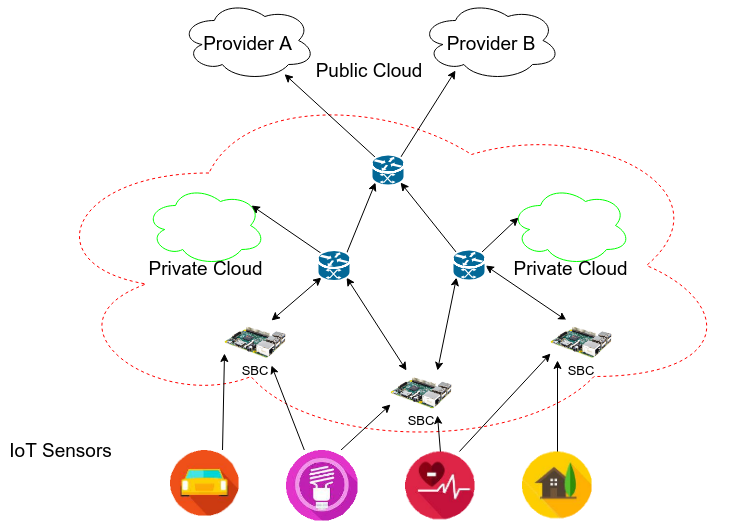
\includegraphics[width=0.5\linewidth]{figures/cassalesimgs-000.png}
    \caption{\arch \cite{Cassales2019a} physical architecture and deployment scenario overview.}
    \label{fig:mfog-phy-arch-cloud}
\end{figure}

This paper is organized as follows:
% Section \ref{sec:related} presents the related works.
Section \ref{sec:minas} reviews the chosen \nd algorithm \minas.
A distributed extension of \minas, including its
implementation and evaluation are presented in Section \ref{sec:prop}
and in Section \ref{sec:experiments} we show how we evaluated \mfog and
the discuss results we found.
Finally, Section \ref{sec:conclusion} summarizes the main findings and presents
possible future work.

% \todo{Parei aqui a redação da Introdução.Deixei grifado em vermelho o
% paragrafo que fala das contribuições. Talvez com um pequeno esforço em
% especificar uma versão distribuida do MINAS teriamos uma extensão do mesmo. }

% Desafios de arquitetura e validação:

% - Construção de um protótipo da arquitetura IDSA-IoT:
%   - Kafka (Python): Distribuição e balanceamento pelo cluster kafka, hipótese refutada.
%   - Flink (Java ou Scala): Execução do cluster nos dispositivos de névoa, hipótese refutada.
%   - MPI (C e Python): Execução do cluster nos dispositivos de névoa, hipótese aceita.
% - Reimplementação do algoritmo MINAS com fidelidade:
%   - Duas versões: a descrita e a implementação de referência (em Java).
%   - Resolução: utilizar a descrição, não *seguir* a imp. referência, apenas como ponto de comparação. Exemplos:
%     - Definição de raio `r = f * σ` (fator vezes desvio padrão) para `r = max(distance)` (distância máxima);
%     - Tamanho do buffer de desconhecidos e frequência de execução do passo de detecção de novidade;

% \begin{highlight}
% Expected results:
% A system that embraces and explores the inherent distribution of fog computing
% in a IoT scenario opposing regular systems where data streams are collected and
% centralized before processing;
% Impact assessment of the impact of distributed, regional flow characteristics,
% local vs global vs distributed forgetting mechanism and other polices.

% IDS characteristics and description of physical scenario.

% MINAS characteristics.

% Distribution and IDSA-IoT architecture.
% \end{highlight}

% This paper is structured as follows:
% Section \ref{sec:related} presents previous works that addresses related
% problems and how they influenced our solution.
% Section \ref{sec:implementation} address our proposal, the work done, issues
% found during implementation and discusses parameters and configurations options
% and how we arrived at our choices.
% Section \ref{sec:experiments} shows experiments layouts and results, we
% compare serial and distributed implementation's metrics for validation,
% we also evaluate communication delay effects on classification metrics and
% conclude with the speedup per core and overall maximum stream speed.
% Section \ref{sec:conclusion} summarizes the research results and presents our
% final conclusions and future works.
